\documentclass[t,aspectratio=169]{beamer}
\usepackage[utf8]{inputenc}
\usepackage[T1]{fontenc}
\usepackage{xcolor}
\usepackage{hyperref}
\usepackage{tikz}
\usepackage{tikz-cd}
\usepackage{pgfplots}
\pgfplotsset{compat=1.8}
\usepackage{adjustbox}
\usepackage{tabularx}
\usepackage{array}
\usepackage{fontspec}
\usefonttheme{serif} % default family is serif
\usepackage{hyperref}

\title{Multimodal MCMC with Replica Exchange and TensorFlow Probability}
\date{Bayesian Mixer London, Nov 30, 2020}
\author{Simeon Carstens}
\newcommand{\todo}{\textcolor{red}{\textbf{TODO}}}
\renewcommand{\d}{\mathrm{d}}
\newcommand{\btVFill}{\vskip0pt plus 1filll}
\setmainfont{Roboto}
\usetheme{tweag}

\begin{document}

\begin{frame}
  \titlepage
\end{frame}

\begin{frame}
  \frametitle{Tweag I/O}
  Software engineering lab based in Paris with employees all around the world.\\
  \bigskip
  We specialize in
  \begin{itemize}
  \item software engineering, with a focus on functional programming
  \item DevOps, with a focus on reproducible software systems and builds
  \item data science -- from the first model to production deployment
  \end{itemize}
  Industries: among others finance, biotech, automotive\\
  \bigskip
  Need help with your project? Want to work with us?\\
  \bigskip
  \centering
  www.tweag.io\\
  \bigskip
  hello@tweag.io
\end{frame}

\begin{frame}
  \frametitle{Multimodality}
  \begin{columns}
    \begin{column}{0.48\textwidth}
      Unimodal distribution:
      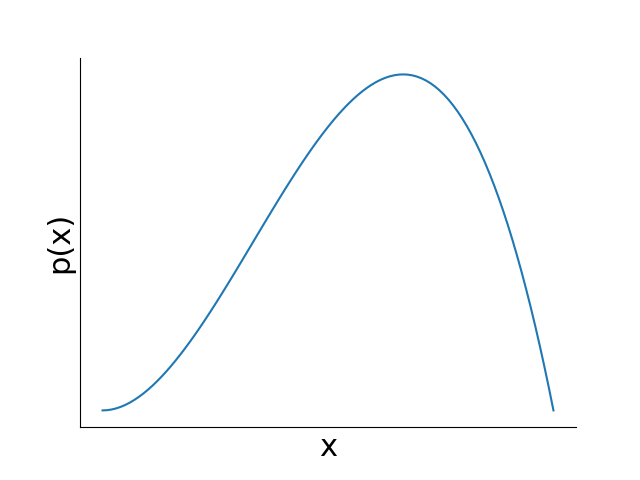
\includegraphics[width=0.8\textwidth]{images/unimodal}
    \end{column}
    \begin{column}{0.48\textwidth}
      Bimodal distribution:
      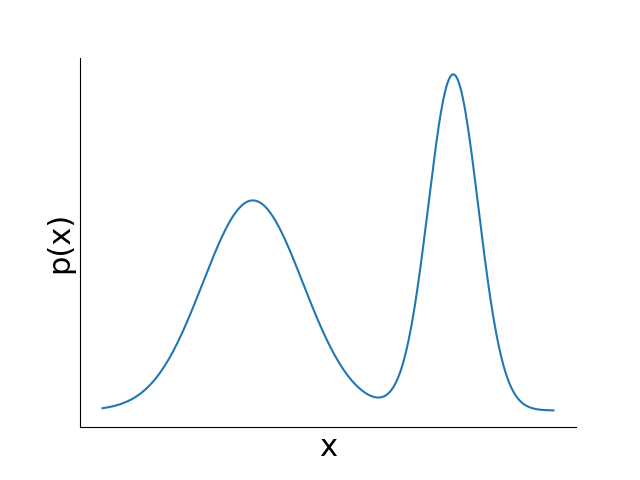
\includegraphics[width=0.8\textwidth]{images/bimodal}
    \end{column}
  \end{columns}
\end{frame}

\begin{frame}
  \frametitle{Multimodality: common occurences}
  \begin{description}
  \item[mixture models] \hfill \\
    For GMM parameterized by mixture weight $\theta$ and $\mu_1, \mu_2, \sigma$:
    \begin{equation*}
      p(\theta, \mu_1, \mu_2, \sigma|y) = p(1-\theta, \mu_2, \mu_1, \sigma|y)
    \end{equation*}
  \item[models invariant under reflections] \hfill \\
    e.g., biomolecular structure determination:
    \begin{equation*}
     L(\mathbf x_1, \ldots \mathbf x_N) = p(D|\mathbf x_1, \ldots \mathbf x_N) = L(\ldots, |\mathbf x_i - \mathbf x_j| \ldots)
    \end{equation*}
  \item[latent variable models] \hfill \\
    e.g., probabilistic PCA: symmetry w.r.t. rotation of latent variable coordinates
  % \item[overparameterized models]
  \end{description}
\end{frame}

\begin{frame}
  \frametitle{Refresher: Metropolis-Hastings}
  \begin{columns}
  \begin{column}{0.48\textwidth}
  \begin{tcolorbox}[fontupper=\small, title=Markov chain]
    Random process with
    \begin{equation*}
      p(x_{i+1}|x_i, x_{i-1}, \ldots, x_1) = p(x_{i+1}|x_i)
    \end{equation*}
    $\rightarrow$ a Markov chain has no ``memory''\\
    
    In some conditions: converges to a unique invariant distribution $\pi(x)$
  \end{tcolorbox}  
\end{column}
\begin{column}{0.48\textwidth}  
  \begin{tcolorbox}[fontupper=\small, title=Metropolis-Hastings algorithm]
    %\tcblower
    Construct Markov chain with invariant distribution $\pi(x)=p(x)$:
    \begin{enumerate}
    \item starting at state, $x_i$, propose a new state $x_{i+1}^*$ from $q(x_{i+1}^*|x_i)$
    \item calculate acceptance probability $p_{\mathrm{acc}}$
    \item draw $u \sim \mathcal U(0,1)$
    \item if $u < p_{\mathrm{acc}}$: $x_{i+1} = x_{i+1}^*$, else $x_{i+1} = x_i$
    \end{enumerate}
  \end{tcolorbox}
\end{column}
\end{columns}
\end{frame}

\begin{frame}{Metropolis (-Hastings)}
  Initialize with any state $x_0$\\
  \adjustbox{valign=t}{
  \begin{minipage}{0.45\linewidth}
    \par
    \noindent\phantom{\parbox{\linewidth}{%
    \begin{enumerate}
    \item calculate a proposal state $x_1^*$ by randomly perturbing $x_0$
    \item calculate acceptance probability
      \[p_\mathrm{acc}=\min\left(\frac{p(x_1^*)}{p(x_0)}, 1\right)\]
    \item with probability $p_\mathrm{acc}$, accept proposal state $x_1^*$ as the next state $x_1$, else copy $x_0$
    \end{enumerate}
    }}\par
    \vfill
    Sequence of states:\\
    $(x_0)$
  \end{minipage}}
  \hfill
  \adjustbox{valign=t}{
  \begin{minipage}{0.45\linewidth}
    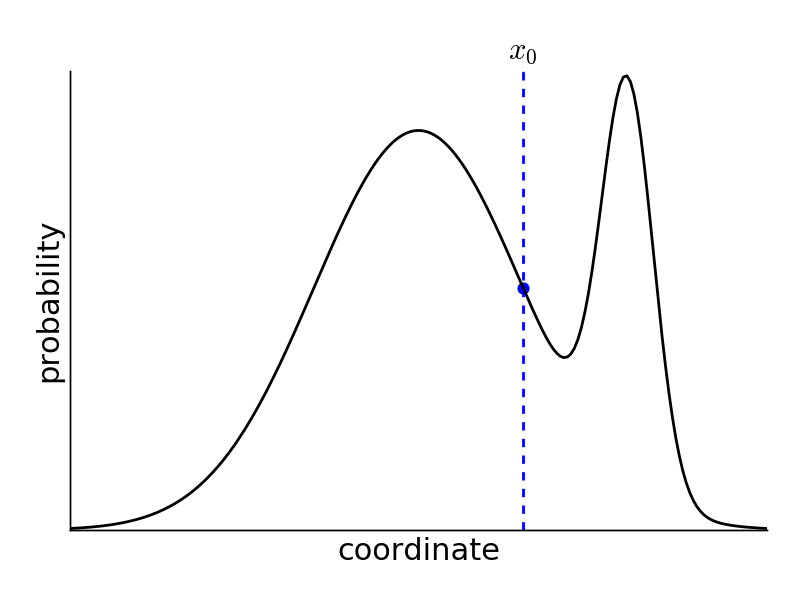
\includegraphics[width=1.0\linewidth]{images/rwmc/03}
  \end{minipage}}
  \btVFill  
  \hfill \scriptsize Metropolis et al., J. Chem. Phys (1953); Hastings, Biometrika (1970)\smallskip
\end{frame}


\begin{frame}{Metropolis (-Hastings)}
  Initial state: $x_0$\\
  \adjustbox{valign=t}{
    \begin{minipage}{0.45\linewidth}
      \small
    \begin{enumerate}[<+->]
    \item calculate a proposal state $x_1^*$ by randomly perturbing $x_0$
    \item calculate acceptance probability
      \[p_\mathrm{acc}=\min\left(1, \frac{p(x_1^*)}{p(x_0)}\right)\]
    \item with probability $p_\mathrm{acc}$, accept proposal state $x_1^*$ as the next state $x_1$, else copy $x_0$
    \end{enumerate}
    \vfill
    \onslide<3>{\hbox{Sequence of states:}
      $(x_0, x_1)$}
  \end{minipage}}
  \hfill
  \adjustbox{valign=t}{
  \begin{minipage}{0.45\linewidth}
     \includegraphics<1>[width=1.0\linewidth]{images/rwmc/04}
     \includegraphics<2>[width=1.0\linewidth]{images/rwmc/05}
     \includegraphics<3>[width=1.0\linewidth]{images/rwmc/06}
  \end{minipage}}
  \btVFill  
  \hfill \scriptsize Metropolis et al., J. Chem. Phys (1953); Hastings, Biometrika (1970)\smallskip
\end{frame}


\begin{frame}{Metropolis (-Hastings)}
  Current state: $x_1$\newline
  \adjustbox{valign=t}{
    \begin{minipage}{0.48\linewidth}
      \small
    \begin{enumerate}[<+->]
    \item calculate a proposal state $x_2^*$ by randomly perturbing $x_1$
    \item calculate acceptance probability
      \[p_\mathrm{acc}=\min\left(1, \frac{p(x_2^*)}{p(x_1)}\right)\]
    \item with probability $p_\mathrm{acc}$, accept proposal state $x_2^*$ as the next state $x_2$, else copy $x_1$
    \end{enumerate}
    \vfill
    \only<3>{Sequence of states:\\
      $(x_0, x_1, x_2)$}
    \only<4>{Sequence of states:\hfill \\
      $(x_0, x_1, x_2, \ldots, x_n)$}
  \end{minipage}}
  \hfill
  \adjustbox{valign=t}{
  \begin{minipage}{0.45\linewidth}
     \includegraphics<1>[width=1.0\linewidth]{images/rwmc/07}
     \includegraphics<2>[width=1.0\linewidth]{images/rwmc/08}
     \includegraphics<3>[width=1.0\linewidth]{images/rwmc/09}
     \includegraphics<4>[width=1.0\linewidth]{images/rwmc/18}
  \end{minipage}}
  \btVFill  
  \hfill \scriptsize Metropolis et al., J. Chem. Phys (1953); Hastings, Biometrika (1970)\smallskip
\end{frame}

\begin{frame}
  \frametitle{Multimodality: hard to sample}
  Markov chain can get stuck in modes:
  \bigskip
  \begin{columns}
    \begin{column}{0.4\textwidth}
      Lucky us:\\
      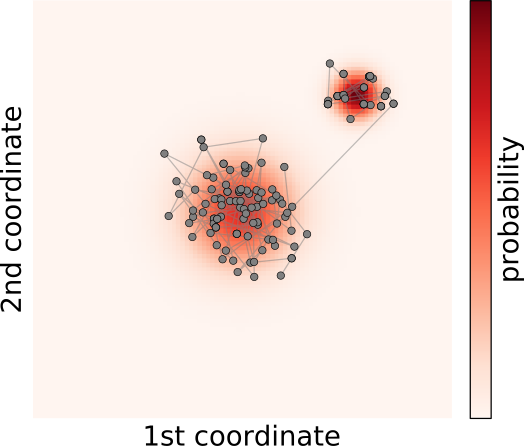
\includegraphics[width=0.8\textwidth]{images/dist_2d_chain}
    \end{column}
    \begin{column}{0.4\textwidth}
      Unlucky us:\\
      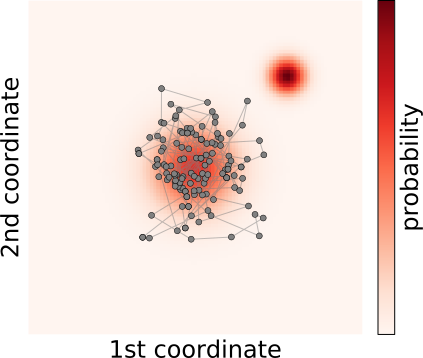
\includegraphics[width=0.8\textwidth]{images/dists_2d_chain_stuck}
    \end{column}
  \end{columns}
  \bigskip
  In higher dimensions: long time until all modes are discovered, if ever
\end{frame}

\begin{frame}
  \frametitle{Replica Exchange}
  Simulate ``flatter'' versions of probability distribution\only<1>{...}\only<2-3>{ and exchange states between Markov chains}\\
  \begin{center}
    \includegraphics<1>[width=0.5\textwidth]{movies_lowq/re/tmp00003}
    \includegraphics<2>[width=0.5\textwidth]{movies_lowq/re/tmp00004}
    \includegraphics<3>[width=0.5\textwidth]{movies_lowq/re/tmp00005}
  \end{center}
\end{frame}

\begin{frame}[fragile]
  \frametitle{Replica Exchange: acceptance criterion (informal motivation)}
  Plain exchanges disturb equilibrium distributions\\
  $\rightarrow$ correct with acceptance criterion\\
  \begin{center}
  \begin{tikzcd}[column sep=2cm, row sep=normal]
    {p_i(x)\mathrm{:} \ \ \ } x_{k-1}^i \arrow[r] & x_k^i \onslide*<1>{\arrow{dr}{p_{i\rightarrow j}}} & x_{k+1}^i \arrow[r]  & x_{k+2}^i\\
    {p_j(x)\mathrm{:} \ \ \ } x_{k-1}^j \arrow[r] & x_k^j \onslide*<2>{\arrow{ur}{p_{j\rightarrow i}}} & x_{k+1}^j \arrow[r,""]  & x_{k+2}^j
  \end{tikzcd}
  \end{center}
  \bigskip
  \begin{columns}
    \begin{column}{0.48\textwidth}
      Probability of accepting $x_k^i$ as ($k+1$)st state of $p_j(x)$ chain:
      \begin{equation*}
        p_{i\rightarrow j}=\frac{p_j(x_k^i)}{p_j(x_k^j)}
      \end{equation*}
    \end{column}
    \begin{column}{0.48\textwidth}
      \onslide<2>{Probability of accepting $x_k^j$ as ($k+1$)st state of $p_i(x)$ chain:
        \begin{equation*}
          p_{j\rightarrow i}=\frac{p_i(x_k^j)}{p_i(x_k^i)}
        \end{equation*}
      \end{column}
    \end{columns}
  }
\end{frame}

\begin{frame}[fragile]
  \frametitle{Replica Exchange: acceptance criterion (informal motivation)}
  Multiply $p_{i\rightarrow j}$ and $p_{j\rightarrow i}$:
  \begin{tcolorbox}[title=General acceptance criterion]
    \begin{equation*}
      p_{\mathrm{acc}}= \mathrm{min}\Bigg\{1, \frac{p_i(x^j)}{p_i(x^i)} \times \frac{p_j(x^i)}{p_j(x^j)}\Bigg\}
    \end{equation*}
  \end{tcolorbox}
  \begin{columns}
    \begin{column}[T]{0.5\textwidth}
      Common case with $p_i(x)\propto \mathrm{e}^{-\beta_i E(x)}$:
      \begin{equation*}
        p_{\mathrm{acc}} = \mathrm{min}\bigg\{1, \mathrm{e}^{(\beta_i-\beta_j)(E(x^i)-E(x^j))}\bigg\}
      \end{equation*}
    \end{column}
    \begin{column}[T]{0.43\textwidth}
      \begin{tcolorbox}[title=Physics terms]
        $\beta$: ``inverse temperature''\\
        $E(x)=-\log p(x)$: ``energy''
      \end{tcolorbox}
    \end{column}
  \end{columns}
  \bigskip
  \textcolor{red}{The more different $\beta_i$ and $\beta_j$, the lower $p_{\mathrm{acc}}$!}
\end{frame}

\begin{frame}
  \frametitle{Replica Exchange: choosing swap partners}
  Choose swap partners such that all replicas are connected, for example:
  \begin{center}
    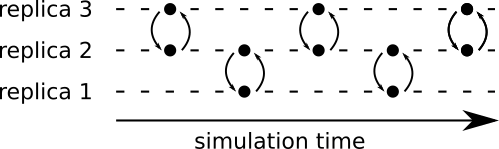
\includegraphics[width=0.6\textwidth]{images/good_swap_strategy}
  \end{center}
  \begin{description}
  \item[Deterministic even-odd swapping:] try to swap $(\mathbf 0, 1), (\mathbf 2, 3), \ldots$ (even), then $(\mathbf 1,2), (\mathbf 3,4), \ldots$ (odd)
  \item[Stochastic even-odd swapping:] decide randomly whether to swap even or odd
  \end{description}
\end{frame}

\begin{frame}
  \frametitle{Replica Exchange: life of a state}
  States have to traverse the ``temperature ladder'' to be useful:
  \begin{center}
    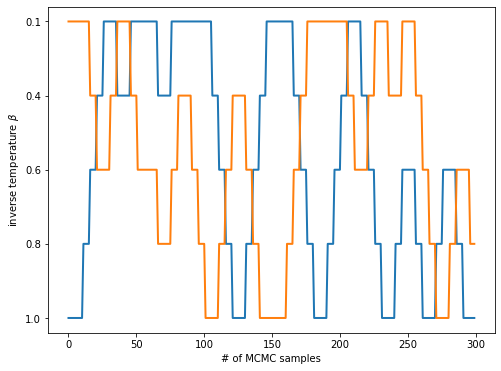
\includegraphics[width=0.4\textwidth]{images/state_trajectories}
  \end{center}
  Stochastic swap scheme: traversal time $\propto (\#\mathrm{\ replicas})^2$ (diffusive)\\
  Deterministic swap scheme: better scaling (non-diffusive)\\
  \bigskip
  In general: \textcolor{red}{more replicas $\nRightarrow$ better sampling}
\end{frame}

\begin{frame}
  \frametitle{Replica Exchange in TensorFlow Probability}
  \centering
  \vfill
  \Huge -- demo time --
  \vfill
\end{frame}

\begin{frame}
  \frametitle{Knobs to tune}
  \begin{itemize}
  \item choice of distribution family $p_i(x)$:
    \begin{itemize}
    \item[--] informed by structure of the sampling problem
    \item[--] in Bayesian inference often morphes posterior into prior 
    \end{itemize}
  \item number of interpolating distributions:\\
    \begin{itemize}
    \item[--] set target acceptance rate ($\approx 23\%$)
    \item[--] heuristics (e.g., constant KL divergence between neighbors)
    \item[--] hardware constraints
    \end{itemize}
  \item frequency of swap attempts:\\
    ``often''
  \item choice of swap partners
  \end{itemize}
\end{frame}

\begin{frame}
  \frametitle{Application: Bayesian determination of chromosome structures}
  \begin{center}
    \includegraphics[width=0.7\textwidth]{images/genome_organization}
  \end{center}
  Structure in ``?'' regime:
  \begin{itemize}
  \item active / passive chromatin compartments
  \item globular domains of several $\approx 100$ nanometers in size
  \end{itemize}
\end{frame}

\begin{frame}
  \frametitle{Bayesian chromosome structure determination}
  \begin{columns}
    \begin{column}[T]{0.28\textwidth}
      \includegraphics[width=\textwidth]{images/schic_matrix}
    \end{column}
    \begin{column}[T]{0.7\textwidth}
      \textbf{Data:}\\
      Binary contacts between loci; model with ``logistic regression'':
      \begin{equation*}
        p(\mathrm{contact\ } i \leftrightarrow j|\vec x_i, \vec x_j) = \frac{1}{1+\mathrm e^{-\alpha (d_{\mathrm{c}} - |\vec x_i - \vec x_j|)}}
      \end{equation*}
    \end{column}
  \end{columns}
  \vfill
  \begin{columns}
    \begin{column}[T]{0.28\textwidth}
      \includegraphics[width=\textwidth]{images/bead_model_schic}
    \end{column}
    \begin{column}[T]{0.7\textwidth}
      \textbf{Prior:}\\
      beads-on-a-chain with volume exclusion $E_\mathrm{ve}(\vec X)$ and chain connectivity $E_\mathrm{nb}(\vec X)$\\
      \bigskip
      Tempered family of posteriors:\\
      \begin{equation*}
        p_i(\vec X|D) \propto [p(D|\vec X)]^{\beta_i} \times \mathrm e^{-E_\mathrm{ve}(\vec X)} \times e^{-E_\mathrm{nb}(\vec X)}
      \end{equation*}
    \end{column}
  \end{columns}
\end{frame}

\begin{frame}
  \frametitle{Application: Bayesian determination of chromatin structures}
  Structures obtained from posterior sampling show several clusters:
  \begin{center}
    \includegraphics[width=0.7\textwidth]{images/schic_structures}
  \end{center}
   Largest clusters: $\approx$ partial mirror images of each other
\end{frame}

\begin{frame}
  \frametitle{Keywords for further reading}
  \begin{description}
  \item[Replica Exchange with Non-equilibrium Switches (RENS):] \hfill \\
    use non-equilibrium switching trajectories to increase acceptance rates
  \item[Recycle RE samples:] \hfill \\
    use histogram reweighting to calculate evidences and automatically tune interpolating distributions
  \item[Multidimensional Replica Exchange:] \hfill \\
    vary not one, but several ``temperatures''
  \end{description}
\end{frame}


\end{document}
